\section{Data Preprocessing and Feature Engineering}

\begin{frame}{Preprocessing \& Feature Engineering}
    \textbf{Missing Values Check:} Zero missing data across all splits (\texttt{isnull().sum()}).
    \vspace{0.3cm}
    
    \textbf{Advanced Feature Engineering:}
    \begin{itemize}
        \item \textbf{Temporal:} \texttt{is\_clutch\_time}, \texttt{is\_buzzer\_beater}.
        \item \textbf{Contextual \& Spatial:} \texttt{is\_home}, \texttt{shot\_angle} (visual perspective).
        \item \textbf{Matrix Cleanup:} Removed redundant (\texttt{lat}, \texttt{lon}) and ID variables.
    \end{itemize}
\end{frame}

\begin{frame}{Categorical Encoding: Target Encoding}
    \textbf{Why Target Encoding?}
    \begin{itemize}
        \item Avoids massive sparse matrices (One-Hot Encoding).
        \item Replaces textual categories with historical probability of success.
    \end{itemize}
    \vspace{0.3cm}
    \textbf{Strict Implementation:}
    \begin{itemize}
        \item Calculated \textbf{exclusively} on the Training Set.
        \item \textbf{Fallback Mechanism:} Unseen categories assigned the \texttt{global\_mean} of the training set to prevent errors.
    \end{itemize}
\end{frame}

\begin{frame}{Correlation Analysis}
    \begin{columns}
        \begin{column}{0.4\textwidth}
            \textbf{Pearson Matrix:}
            \begin{itemize}
                \item Checked linear relationships between engineered features.
                \item \textbf{Result:} Confirms absence of extreme multicollinearity.
                \item Ensures stability of classification algorithms.
            \end{itemize}
        \end{column}
        \begin{column}{0.6\textwidth}
            \begin{figure}
                \centering
                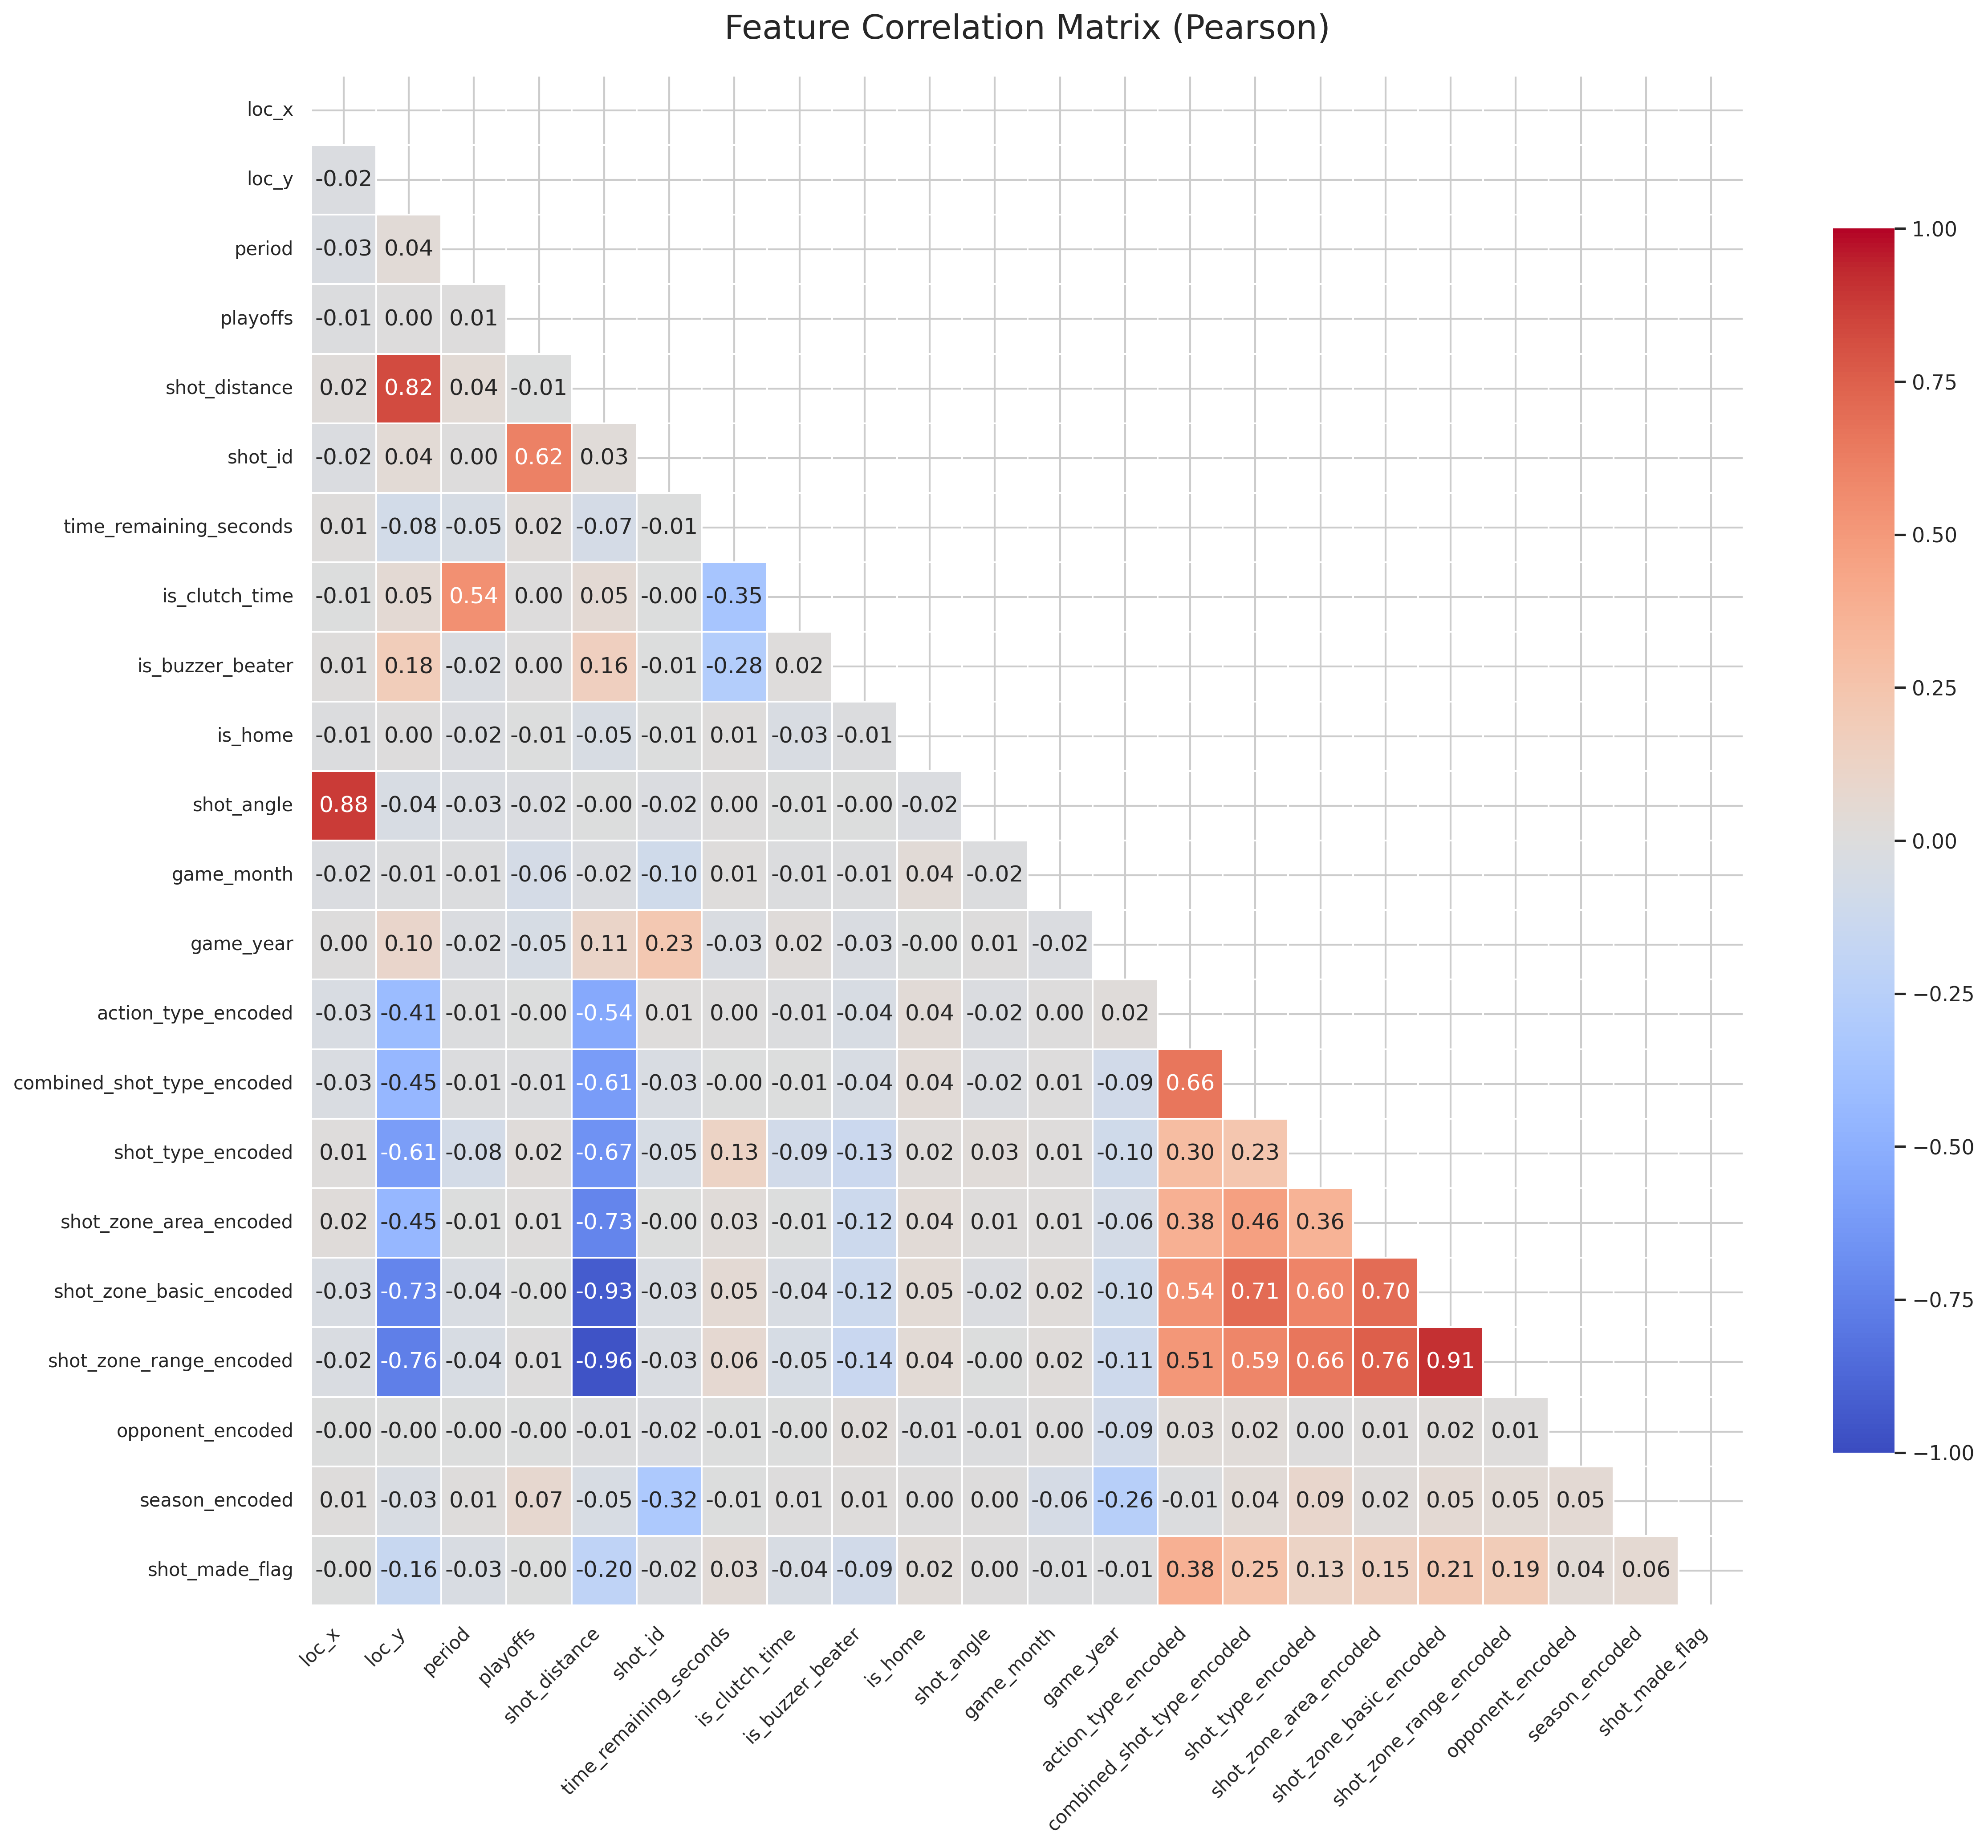
\includegraphics[width=\textwidth]{img/corr_matrix.png}
            \end{figure}
        \end{column}
    \end{columns}
\end{frame}